% vim: set textwidth=78 autoindent:

%\subsection{OGR Converter Plugin}
\subsection{Extension OGR pour la conversion}
% when the revision of a section has been finalized, 
% comment out the following line:
%\updatedisclaimer

%The OGR layer converter plugin allows to convert vector data from one OGR-supported 
%vector format to another OGR-supported vector format. It is very simple to handle and 
%provides functionalities as shown in Figure \ref{fig:ogrconverter_dialog}. The 
%supported formats can vary according to the installed GDAL/OGR package.
L'extension de conversion de couche OGR vous permet de convertir des données vecteurs d'un format supporté par la librairie OGR
vers un autre format supporté par la librairie OGR. Il est très simple à manipuler et vous donne accès à des fonctionnalités
comme montré sur la Figure \ref{fig:ogrconverter_dialog}. Les formats supportés peuvent varier en fonction de la version GDAL/OGR installée.


\begin{itemize}
%\item \textbf{Source Format/Datset/Layer}: Enter OGR format and path to the vector file to be converted
\item \textbf{Source Format/Datset/Layer}: Choississez le format OGR et donnez le chemin vers le fichier à convertir
%\item \textbf{Target Format/Datset/Layer}: Enter OGR format and path to the vector output file
\item \textbf{Target Format/Datset/Layer}: Choississez le format OGR de sortie ainsi que l'emplacement du fichier de sortie
\end{itemize}

\begin{figure}[ht]
   \begin{center}
   %\caption{OGR Layer Converter Plugin \nixcaption}\label{fig:ogrconverter_dialog}\smallskip
   \caption{Convertisseur de couche OGR \nixcaption}\label{fig:ogrconverter_dialog}\smallskip
   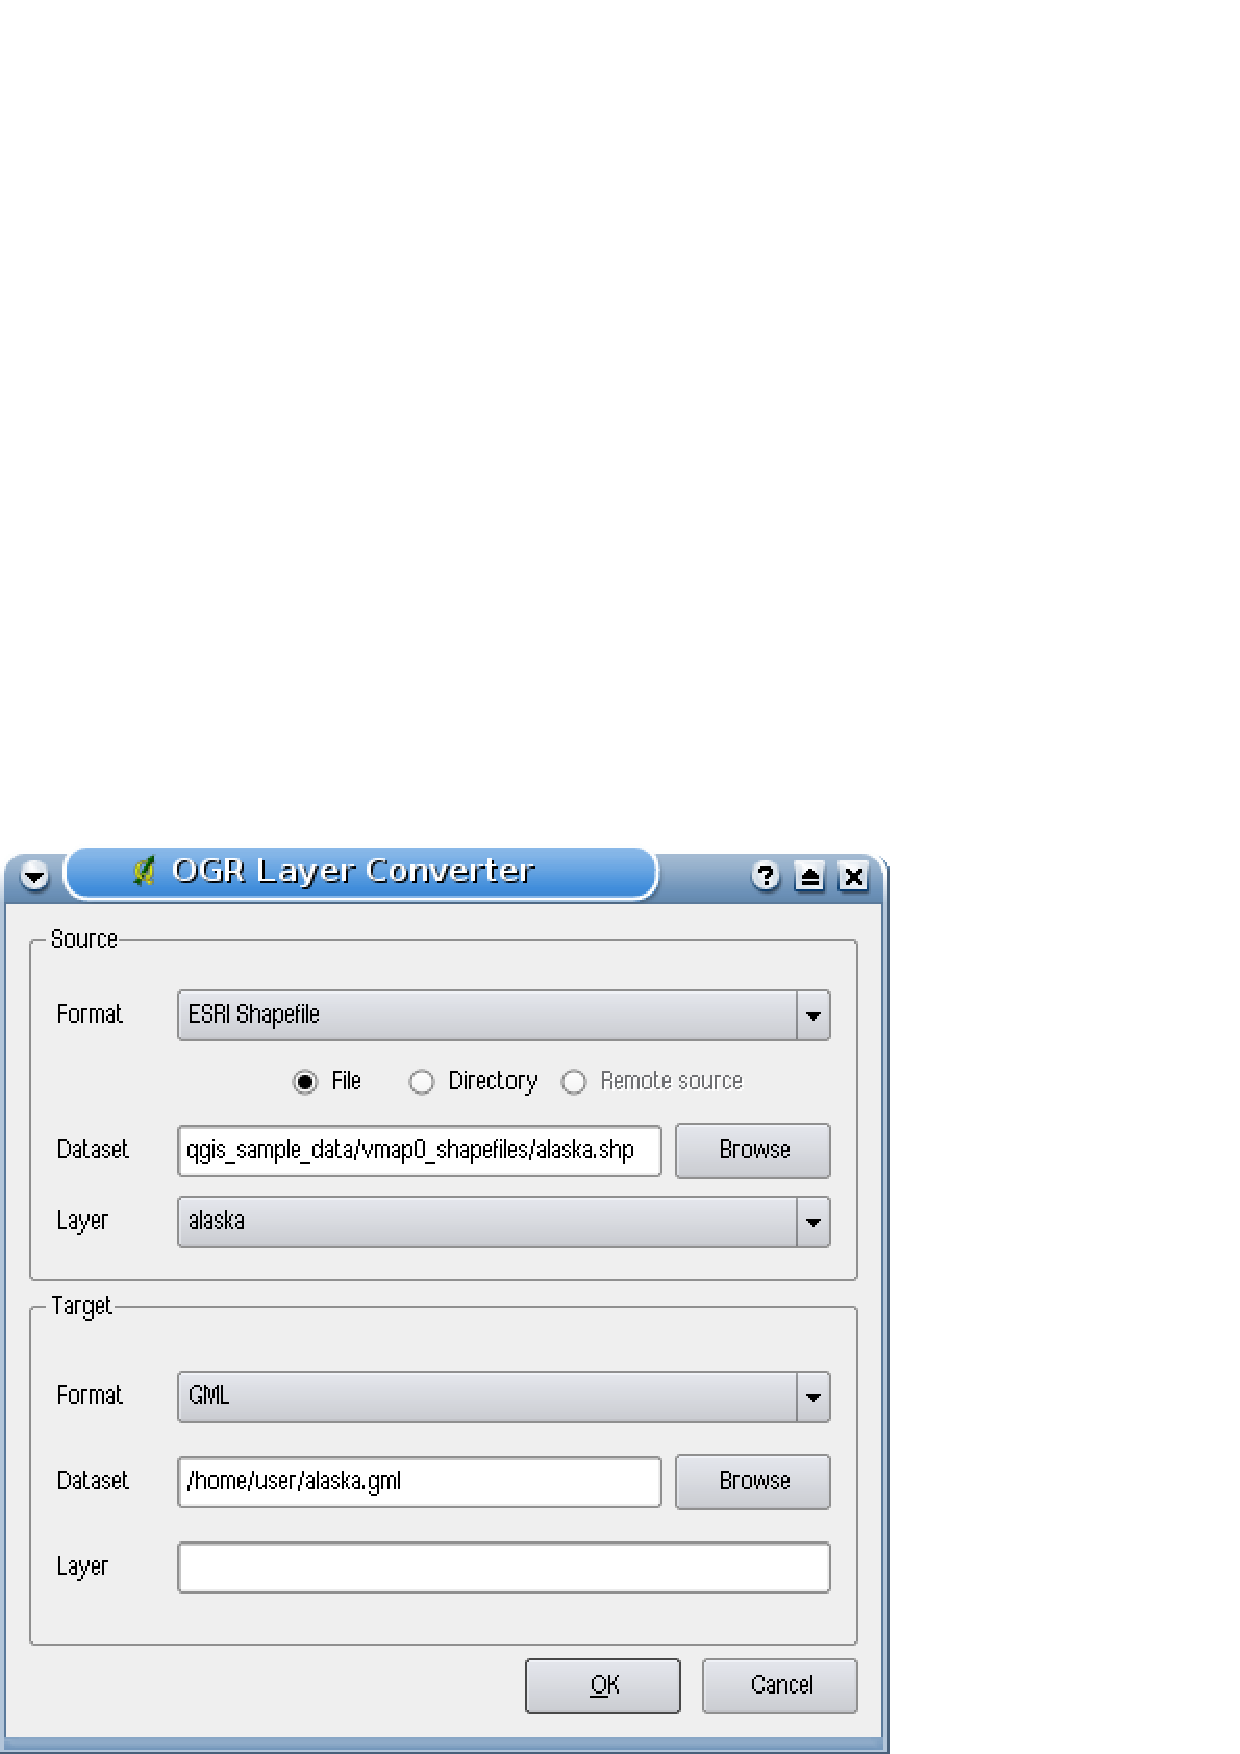
\includegraphics[clip=true, width=9cm]{ogrconverter_dialog}
\end{center}  
\end{figure}

\begin{enumerate}
  %\item Start QGIS, load the OGR converter plugin in the Plugin Manager (see Section 
  \item Démarrez QGIS, chargez le convertisseur OGR dans le gestionnaire de plugin (see Section 
  %\ref{sec:load_core_plugin}) and click on the \toolbtntwo{ogr_converter}{OGR Layer Converter} 
  \ref{sec:load_core_plugin}) et cliquez sur le bouton \toolbtntwo{ogr_converter}{OGR Layer Converter}
  %icon which appears in the QGIS toolbar menu. The OGR Layer Converter plugin dialog appears as shown in Figure \ref{fig:ogrconverter_dialog}.
  qui se trouve dans la barre de menu QGIS. La boite de dialogue convertisseur OGR apparait comme sur la figure \ref{fig:ogrconverter_dialog}.
  %\item Select the OGR-supported format \selectstring{ESRI Shapefile}{\ldots} and the path to the vector input file \filename{alaska.shp} in the Source area.
  \item Sélectionnez le format OGR \selectstring{ESRI Shapefile}{\ldots} et le chemin vers le fichier d'entrée \filename{alaska.shp} dans la partie Source de la boite de dialogue.
  %\item Select the OGR-supported format \selectstring{GML}{\ldots} and define a path and the vector output filename \filename{alaska.gml} in the Target area.
  \item Sélectionnez le format OGR \selectstring{GML}{\ldots} et donnez le chemin ainsi que le nom du fichier de sortie \filename{alaska.gml} dans la partie Cible de la boite de dialogue.
  %\item Click \button{Ok}.
  \item Cliquez sur \button{Ok}.
\end{enumerate}

\newpage